%% ---------------------------------------------------------------------------
%% Flagship INTRODUCTION figure (Figure 1)
%% "Concepts Whisper: Spectral Anti-Concentration and the Dual Geometry
%%  of Transformer Representations" (EMNLP main, camera-ready)
%%
%% Standalone TikZ/PGF -- compile with:  tectonic dual_geometry_v3.tex
%% Produces a tightly-cropped vector PDF; the paper does
%%   \includegraphics{figures/intro/dual_geometry_v3.pdf}
%% and does NOT depend on this file's preamble.
%% ---------------------------------------------------------------------------
\documentclass[tikz,border=2pt]{standalone}

\usepackage[T1]{fontenc}
\usepackage{helvet}
\renewcommand{\familydefault}{\sfdefault}
\usepackage{sansmathfonts}   % sans-serif math to match the modern sans look

\usetikzlibrary{arrows.meta,positioning,calc,backgrounds,shadings,fadings}

% -- Okabe-Ito colorblind-safe palette (groups also differ by SHAPE + POSITION)
\definecolor{head}{HTML}{D55E00}   % vermilion  : vocabulary / high-variance head
\definecolor{headf}{HTML}{F6D3BC}  % light warm fill
\definecolor{tail}{HTML}{0072B2}   % steel blue : activation / low-variance tail
\definecolor{tailf}{HTML}{CDE2EF}  % light cool fill
\definecolor{spec}{HTML}{9AA0A6}   % neutral grey eigen-spectrum
\definecolor{ink}{HTML}{1A1A1A}    % near-black text / arrow
\definecolor{mute}{HTML}{5F6368}   % muted secondary text
\definecolor{grid}{HTML}{C9CDD2}   % faint borders

% ---------------------------------------------------------------------------
% Precomputed, reproducible marker positions (Python/NumPy seed=7).
% HEAD = vocabulary contrasts -> tight cluster (CONCENTRATE), squares.
\def\headpts{2.751/2.050,2.905/2.832,2.607/2.316,2.287/3.086,2.514/3.028,%
2.234/2.857,2.781/2.150,3.447/2.681,2.494/2.926,2.427/3.007,3.005/2.185,%
2.936/2.711,2.805/2.461,2.266/2.546,2.735/3.480,3.112/2.546,2.051/2.934,%
2.512/3.392,1.761/2.658,2.079/2.894}
% TAIL = activation directions -> spread out (ANTI-CONCENTRATE), three methods.
\def\tailO{14.306/2.887,12.157/2.764,14.113/2.435,12.910/3.701,13.502/2.871,%
9.731/4.010,12.339/3.271,12.145/3.300,14.254/3.362,11.295/3.435,12.669/2.436,%
9.544/2.987}                                          % diff-of-means (circle)
\def\tailD{10.589/2.400,11.534/3.756,10.350/3.980,14.813/3.867,10.447/3.232,%
13.096/2.426,10.942/2.516,14.270/3.913,13.041/3.199} % SAE feature (diamond)
\def\tailT{10.247/3.039,14.328/3.191,12.921/2.762,12.504/3.578,11.382/2.198,%
11.584/2.857,10.589/2.208,9.421/2.383,14.282/3.988}  % linear probe (triangle)

% Marker drawing styles (soft rounded, white halo so clusters read cleanly).
\tikzset{
  sq/.style   ={draw=white,line width=0.7pt,fill=head,rounded corners=0.8pt},
  circ/.style ={draw=white,line width=0.7pt,fill=tail},
  dia/.style  ={draw=white,line width=0.7pt,fill=tail,line join=round},
  tri/.style  ={draw=white,line width=0.7pt,fill=tail,line join=round},
}

\begin{document}
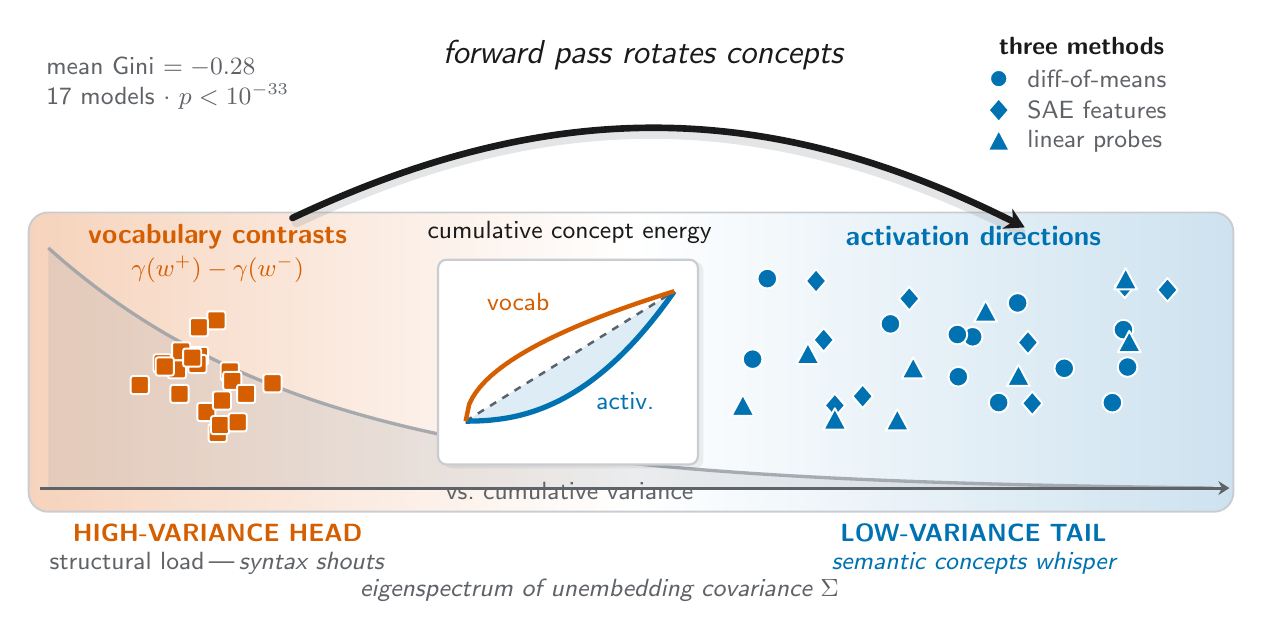
\begin{tikzpicture}[x=1cm,y=1cm]

  %% ==== background region bands: warm head -> quiet centre -> cool tail =====
  \begin{scope}
    \clip[rounded corners=7pt] (0.35,1.05) rectangle (15.65,4.85);
    \shade[left color=headf,right color=tailf,middle color=white]
      (0.35,1.05) rectangle (15.65,4.85);
    % gentle vertical fade toward the top so markers/text stay crisp
    \shade[top color=white,bottom color=white,opacity=0]
      (0.35,1.05) rectangle (15.65,4.85);
  \end{scope}
  \draw[grid,line width=0.7pt,rounded corners=7pt]
      (0.35,1.05) rectangle (15.65,4.85);

  %% ==== grey eigen-spectrum "mountain": loud head -> quiet tail ============
  \path[fill=spec,fill opacity=0.20]
    plot[domain=0:1,samples=160]
      ({0.6+14.8*\x},{1.35+3.05*((exp(-4.2*\x)*(1-0.12*\x)+0.012-0.025)/0.987)})
    -- (15.4,1.35) -- (0.6,1.35) -- cycle;
  \draw[spec,line width=1.2pt,opacity=0.85]
    plot[domain=0:1,samples=160]
      ({0.6+14.8*\x},{1.35+3.05*((exp(-4.2*\x)*(1-0.12*\x)+0.012-0.025)/0.987)});

  %% ==== spectrum axis (high-variance -> low-variance) ======================
  \draw[mute,line width=1.1pt,-{Stealth[length=4pt,width=5pt]}]
      (0.5,1.35) -- (15.6,1.35);

  %% ==== marker clusters ====================================================
  % HEAD: vocabulary contrasts (vermilion squares), concentrated
  \foreach \px/\py in \headpts {
    \fill[sq] (\px-0.115,\py-0.115) rectangle (\px+0.115,\py+0.115);
  }
  % TAIL: activation directions, three independent methods, spread out
  \foreach \px/\py in \tailO { \fill[circ] (\px,\py) circle (0.125); }
  \foreach \px/\py in \tailD {
    \fill[dia] (\px,\py+0.15)--(\px+0.13,\py)--(\px,\py-0.15)--(\px-0.13,\py)--cycle; }
  \foreach \px/\py in \tailT {
    \fill[tri] (\px,\py+0.155)--(\px+0.145,\py-0.115)--(\px-0.145,\py-0.115)--cycle; }

  %% ==== the forward-pass rotation arrow (visual protagonist) ===============
  \draw[spec,line width=3.4pt,opacity=0.28,line cap=round]      % soft shadow
      (3.75,4.72) to[bend left=26] (12.95,4.60);
  \draw[ink,line width=2.4pt,line cap=round,-{Stealth[length=7pt,width=8pt]}]
      (3.7,4.78) to[bend left=26] (13.0,4.66);

  %% ==== headline title above the arc =======================================
  \node[ink,font=\itshape\large] at (8.15,6.85)
      {forward pass rotates concepts};

  %% ==== cluster captions ===================================================
  % head (vermilion vocabulary contrasts -- a real finding)
  \node[head,font=\bfseries\normalsize,align=center] at (2.75,4.55)
      {vocabulary contrasts};
  \node[head,font=\small] at (2.75,4.13) {$\gamma(w^{+})-\gamma(w^{-})$};
  % tail (steel-blue activation directions -- the protagonist)
  \node[tail,font=\bfseries\normalsize] at (12.35,4.55)
      {activation directions};

  %% ==== inset: empirical cumulative-energy signature =======================
  \begin{scope}
    % card
    \fill[black,opacity=0.06,rounded corners=3pt] (5.62,1.60) rectangle (8.92,4.22);
    \filldraw[fill=white,draw=grid,line width=0.8pt,rounded corners=3pt]
        (5.55,1.65) rectangle (8.85,4.25);
    % plot frame: t in [0,1] -> x in [5.90,8.55], y in [2.20,3.85]
    % uniform diagonal
    \draw[mute,line width=0.9pt,dash pattern=on 2.6pt off 2.6pt]
        (5.90,2.20) -- (8.55,3.85);
    % activation curve bows BELOW the diagonal -> anti-concentration
    \path[fill=tail,fill opacity=0.13]
      plot[domain=0:1,samples=60,variable=\t] ({5.90+2.65*\t},{2.20+1.65*pow(\t,2.3)})
      -- (5.90,2.20) -- cycle;
    \draw[tail,line width=1.9pt]
      plot[domain=0:1,samples=60,variable=\t] ({5.90+2.65*\t},{2.20+1.65*pow(\t,2.3)});
    % vocabulary curve bows ABOVE the diagonal -> concentration
    \draw[head,line width=1.6pt]
      plot[domain=0:1,samples=60,variable=\t] ({5.90+2.65*\t},{2.20+1.65*sqrt(\t)});
    % inline curve labels
    \node[head,font=\small,anchor=west] at (6.05,3.72) {vocab};
    \node[tail,font=\small,anchor=east] at (8.42,2.46) {activ.};
    % axis meaning
    \node[ink,font=\small] at (7.22,4.60) {cumulative concept energy};
    \node[mute,font=\small,anchor=north] at (7.22,1.55) {vs.\ cumulative variance};
  \end{scope}

  %% ==== legend: three independent methods (balances the stat, top-right) ===
  \begin{scope}[shift={(12.55,6.55)}]
    \node[ink,font=\small\bfseries,anchor=west] at (0.0,0.42) {three methods};
    \fill[circ] (0.12,0.0) circle (0.11);
    \node[mute,font=\small,anchor=west] at (0.36,0.0) {diff-of-means};
    \fill[dia] (0.12,-0.40+0.15)--(0.25,-0.40)--(0.12,-0.40-0.15)--(-0.01,-0.40)--cycle;
    \node[mute,font=\small,anchor=west] at (0.36,-0.40) {SAE features};
    \fill[tri] (0.12,-0.80+0.15)--(0.26,-0.80-0.115)--(-0.02,-0.80-0.115)--cycle;
    \node[mute,font=\small,anchor=west] at (0.36,-0.80) {linear probes};
  \end{scope}

  %% ==== headline statistic (subtle, top-left) ==============================
  \node[mute,font=\small,align=left,anchor=north west] at (0.45,6.95)
      {mean Gini $=-0.28$\\17 models\,\,$\cdot$\,\,$p<10^{-33}$};

  %% ==== region labels + framing (below the axis) ===========================
  % head: named finding, but the functional "syntax" reading is SECONDARY/muted
  \node[head,font=\small\bfseries] at (2.75,0.78) {HIGH-VARIANCE HEAD};
  \node[mute,font=\small] at (2.75,0.40) {structural load\,---\,\emph{syntax shouts}};
  % tail: the robust protagonist
  \node[tail,font=\small\bfseries] at (12.35,0.78) {LOW-VARIANCE TAIL};
  \node[tail,font=\small\itshape] at (12.35,0.40) {semantic concepts whisper};

  %% ==== axis caption =======================================================
  \node[mute,font=\small\itshape] at (7.6,0.05)
      {eigenspectrum of unembedding covariance $\Sigma$};

\end{tikzpicture}
\end{document}
